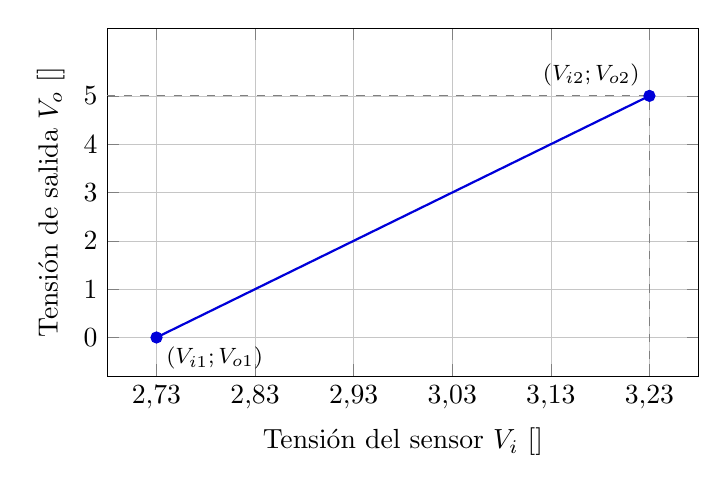
\begin{tikzpicture}
  \begin{axis}[
    width=0.75\textwidth,
    height=6cm,
    grid=both,
    grid style={line width=.1pt, draw=gray!25},
    major grid style={line width=.2pt, draw=gray!45},
    xlabel={Tensión del sensor $V_i$ [\unit{\volt}]},
    ylabel={Tensión de salida $V_o$ [\unit{\volt}]},
    xmin=2.68, xmax=3.28,
    ymin=-0.8, ymax=6.4,
    xtick={2.73, 2.83, 2.93, 3.03, 3.13, 3.23},
    xticklabel style={/pgf/number format/precision=2, /pgf/number format/fixed zerofill, /pgf/number format/use comma},
    ytick={0,1,2,3,4,5},
  ]
    \addplot[thick, color=blue!85!black, domain=2.73:3.23, samples=2] {10*(x-2.73)};
    \addplot[dashed, gray] coordinates {(2.68,5) (3.23,5) (3.23,-0.8)};
    \addplot[only marks, mark=*, color=blue!85!black] coordinates {(2.73,0) (3.23,5)};
    \node[anchor=north west, font=\footnotesize] at (axis cs:2.73,0) {$(V_{i1}; V_{o1})$};
    \node[anchor=south east, font=\footnotesize] at (axis cs:3.23,5) {$(V_{i2}; V_{o2})$};
  \end{axis}
\end{tikzpicture}
